\chapter{Research Design}

\paragraph{}
Our research design has been further refined after the initial design to ensure that the plan for the research helps in properly answering the research questions. High level diagram for the research design is shown in Figure \ref{figure:des}.

\begin{figure}[H]
    \centering
    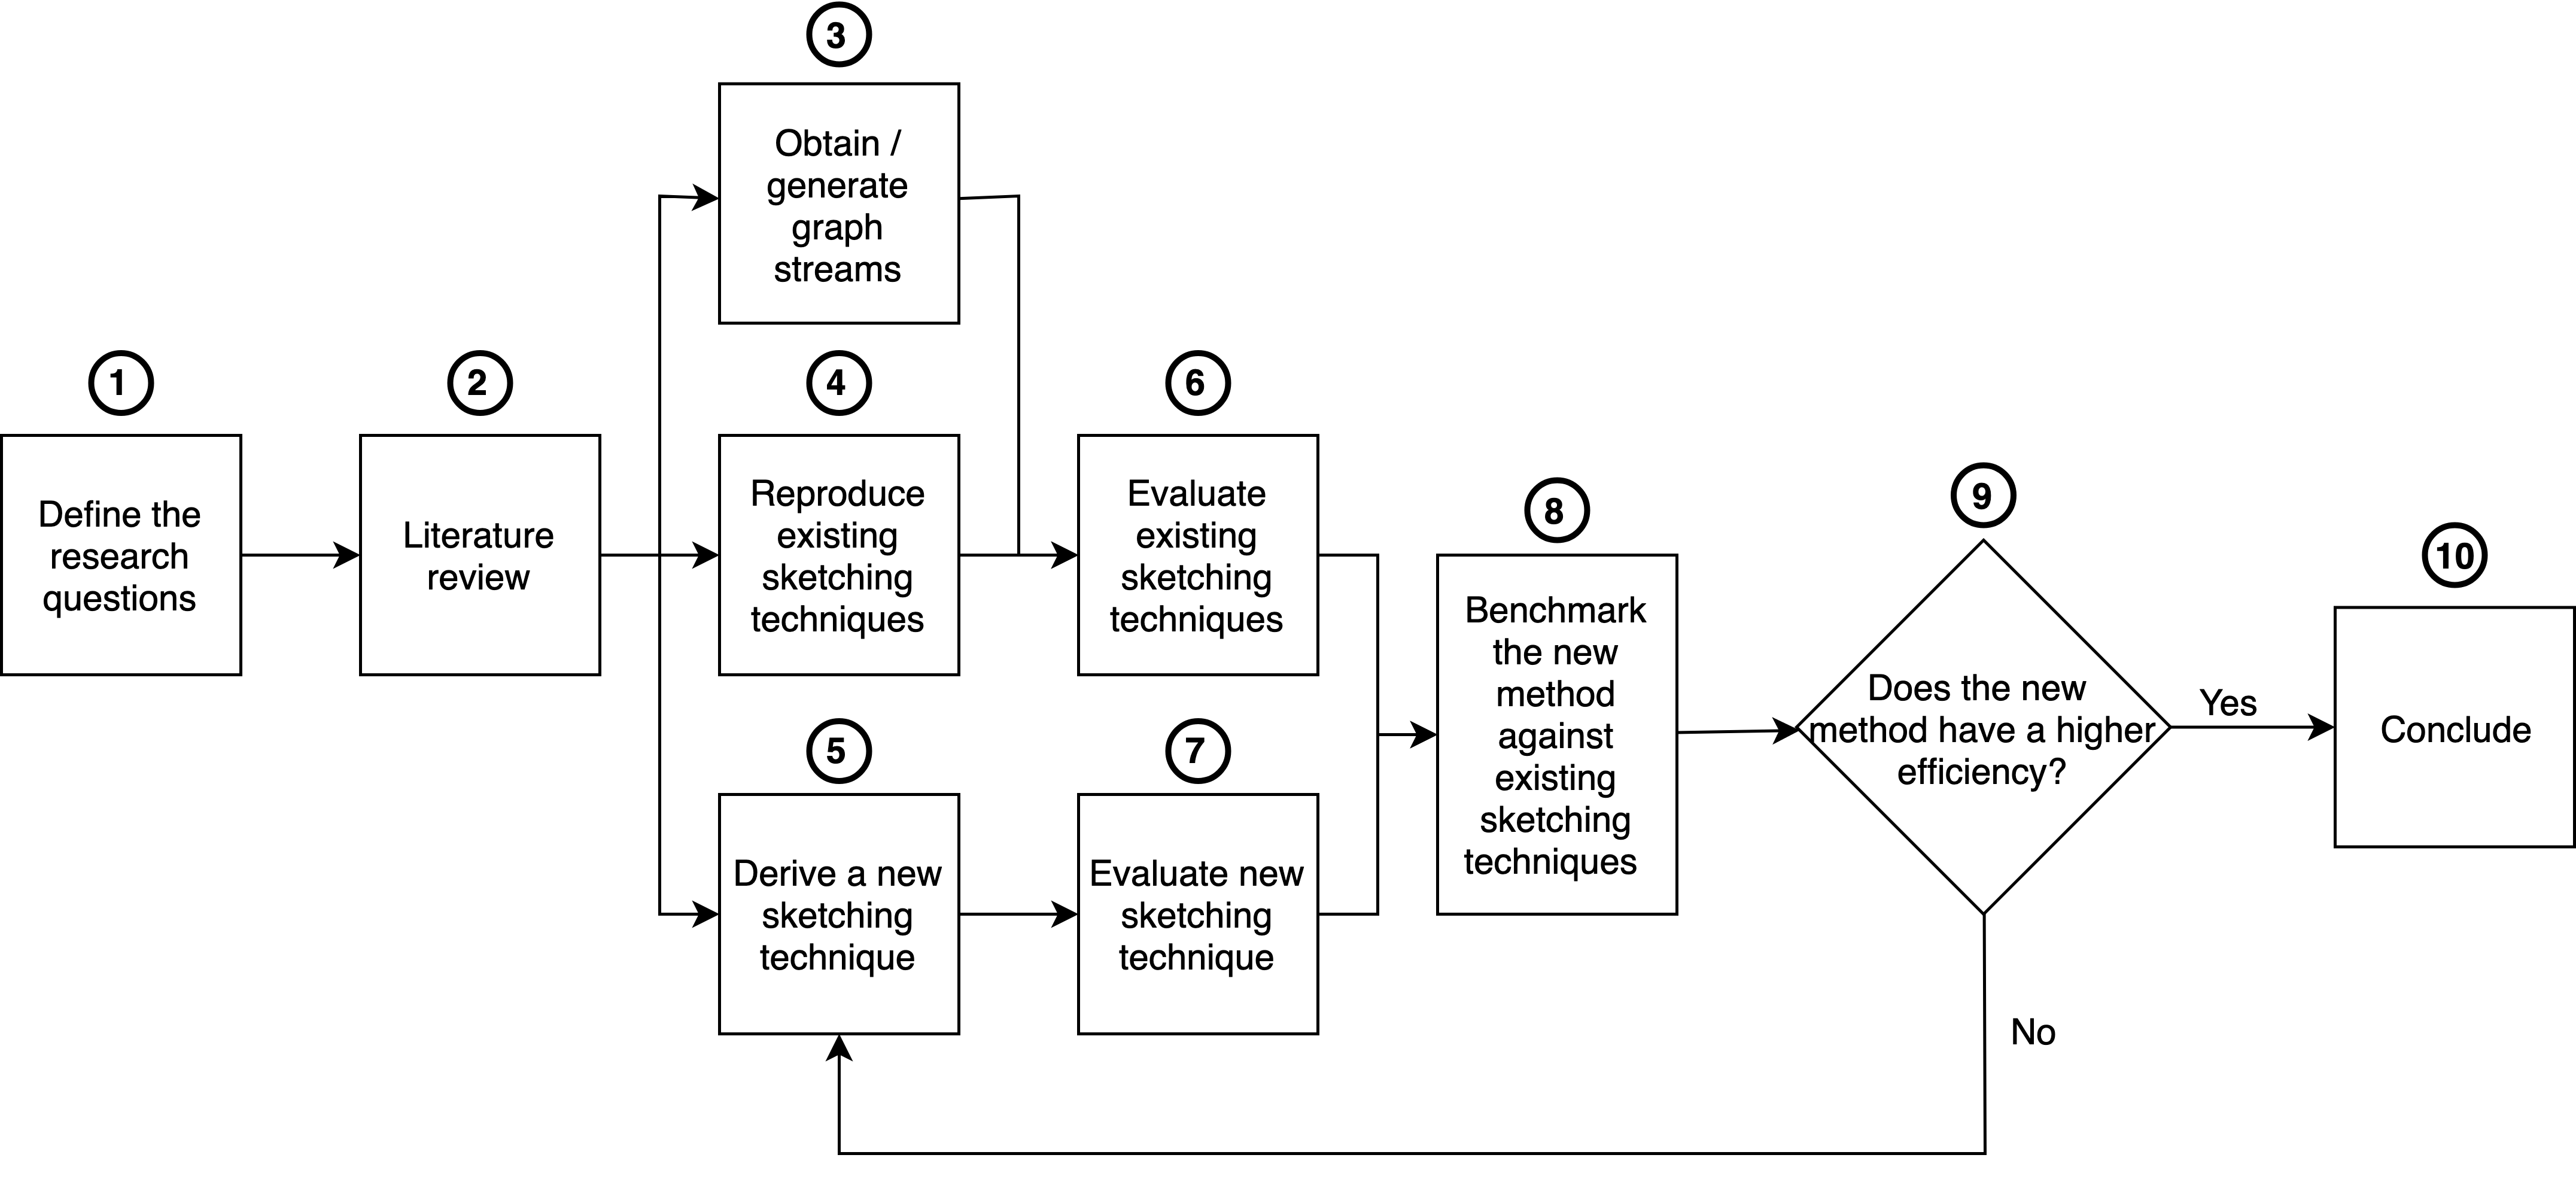
\includegraphics[width=\textwidth]{images/research-design}
    \caption{High level diagram of the research design}
    \label{figure:des}
\end{figure}

\section*{Step 1 - Define the research question}

\paragraph{}
Our research question is,

\begin{itemize}
    \item How to improve upon existing streaming graph sketching techniques such that the graph properties could be identified in realtime? 
\end{itemize}

\paragraph{}
In order to achieve this, a comprehensive literature review on the existing streaming graph sketching techniques would have to be done. This will be done in step 2. 

\section*{Step 2 - Literature review}

\paragraph{}
In this step a literature review will be done on the following areas,

\begin{itemize}
    \item Streaming graphs
    \item Graph sketches and synopses
    \item Graph partitioning
    \item Graph summarization
        \begin{itemize}
            \item General stream summarization techniques
        \end{itemize}
    \item Graph properties
        \begin{itemize}
            \item Real world graph properties
        \end{itemize}
\end{itemize}

\paragraph{}
All the graph summarization techniques that are relevant for this research will be studied in depth. 

\section*{Step 3 - Obtain / generate graph streams}

\paragraph{}
Step 3 will consist of obtaining datasets for the purpose of testing and benchmarking the implementations. Since this research is geared towards general queries, datasets will have to be chosen from different application domains. Few such highly prominent domains are, 

\begin{itemize}
    \item Social network graphs
    \item Computer network activity graphs
    \item Web graphs
\end{itemize}

\section*{Step 4 - Reproduce existing sketching techniques}

\paragraph{}
Existing sketching techniques will be re-implemented. This step is necessary as query results with the results obtained from the proposed sketching technique will have to be compared in order to deduce the strengths and weaknesses of the proposed method. 

\section*{Step 5 - Derive a new sketching technique}

\paragraph{}
In step 5, a new sketching technique will be proposed and implemented after studying all the relevant existing work (step 2). 

\paragraph{}
In addition to implementing the proposed method, its properties and boundaries will be deduced in mathematical form. Theoretical proofs will be devised in order to prove the generalizability of the proposed technique. 

\section*{Step 6 - Evaluate existing sketching techniques}

\paragraph{}
Implemented existing sketching techniques will be benchmarked against selected datasets and the results will be obtained. 

\section*{Step 7 - Evaluate new sketching technique}

\paragraph{}
Proposed sketching technique will be benchmarked against selected datasets and the results will be obtained. 

\section*{Step 8 - Benchmark the new method against existing sketching techniques}

\paragraph{}
In step 8, the results obtained from step 6 and step 7 will be compared to multiple characteristics. 

\paragraph{}
Examples for some evaluation measures are,

\begin{itemize}
    \item Average relative error\cite{kumarage_efficient_2017}
    \item Number of effective queries\cite{kumarage_efficient_2017}
\end{itemize}

Examples for some of the comparisons are,

\begin{itemize}
    \item Compression ratio vs Average relative error
    \item Number of hash functions vs Average relative error
\end{itemize}

More details regarding the evaluation plan will be covered in chapter \ref{evplan}.

\section*{Step 9 - Does the new method have a higher efficiency?}

\paragraph{}
In this step it will be decided whether the newly proposed sketching technique poses considerable accuracy increase or other advantages over the existing techniques. If it does, the process will move step 10. Otherwise the process would move back to step 5 and iterate the same process. 

\section*{Step 10 - Conclude}

\paragraph{}
The research will be concluded with detailing down the characteristics of newly proposed streaming graph summarization technique. The conclusion will also contain a mathematical breakdown of the proposed algorithm and its boundaries. 